\documentclass[review,12pt]{elsarticle}

\usepackage{amsmath,amssymb}
\usepackage{booktabs}
\usepackage{graphicx}
\usepackage{siunitx}
\usepackage[hidelinks]{hyperref}
\usepackage{xcolor}
\usepackage{microtype}
\emergencystretch=1.5em
\newcommand{\todo}[1]{\textcolor{red}{[TODO: #1]}}
\newcommand{\pp}{\,pp}

\journal{Neurocomputing}

\begin{document}

\begin{frontmatter}

\title{Quantized reward-model verifiers in Best-of-N mathematical answer selection:
accuracy, memory and value retention}

\author[a]{Hector Borobia\corref{cor1}}
\ead{hecboar@doctor.upv.es}
\author[b]{Elies Segu\'{i}-Mas}
\ead{eseguim@upvnet.upv.es}
\author[c]{Guillermina Tormo-Carb\'{o}}
\ead{gtormo@omp.upv.es}
\cortext[cor1]{Corresponding author.}

\affiliation[a]{organization={VRAIN -- Valencian Research Institute for Artificial
Intelligence, Universitat Polit\`ecnica de Val\`encia},city={Valencia},country={Spain}}
\affiliation[b]{organization={Department of Economics and Social Sciences, Universitat
Polit\`ecnica de Val\`encia},city={Valencia},country={Spain}}
\affiliation[c]{organization={Department of Business Organisation, Universitat
Polit\`ecnica de Val\`encia},city={Valencia},country={Spain}}

\begin{abstract}
Best-of-$N$ selection with a learned verifier is a simple way to turn inference compute
into accuracy on mathematical reasoning, but the verifier, a reward model of several
billion parameters, competes with the generator for accelerator memory. We ask whether
post-training quantization of the verifier preserves its selections. On frozen pools of
32 candidates per problem (GSM8K and MATH), we compare three outcome reward models (1.7B,
4B, 8B) and a 7B process reward model in BF16, NF4, GPTQ (4 and 3 bits), AWQ and
round-to-nearest, measure memory with packed 4-bit kernels, and fix the analysis plans
before the data exist. Four-bit GPTQ leaves the Best-of-32 accuracy of the 8B model
unchanged (equivalence within $\pm3$ points; 90\% interval $[-0.6, +1.3]$), and the
result replicates in two follow-up studies, with a 7B math generator and with 1,060 new
hard problems, for both reward-model types. Where the verifier beats majority vote,
4-bit quantization keeps most of that advantage (the process reward model retains 93\%
of an 8.2-point advantage). Under a 6~GB verifier budget, a 4B model with packed 4-bit
weights beats the best full-precision verifier that fits by 1.4--2.25 points. The
mechanism is answer redundancy: quantization changes the selected candidate on a quarter
to a third of problems, but the new winner usually carries the same answer; 3-bit
weights and the smallest verifier break down. We also show that a strict answer grader
can turn reward-model format preferences into spurious quantization gains, and that with
a strong generator, majority vote matches or beats reward-model selection on hard
problems.
\end{abstract}

\begin{keyword}
post-training quantization \sep reward models \sep Best-of-N \sep test-time compute
\sep mathematical reasoning \sep preregistration
\end{keyword}

\end{frontmatter}

\section{Introduction}\label{sec:intro}

Sampling several candidate solutions and letting a learned verifier pick one
(Best-of-$N$) is one of the simplest ways to turn extra inference compute into accuracy
on mathematical reasoning \cite{cobbe2021gsm8k,lightman2023verify,snell2024scaling}. The
verifier is usually a reward model with a few billion parameters. An outcome reward
model (ORM) scores a complete response, and a process reward model (PRM) scores each
reasoning step. In deployment the verifier competes with the generator for accelerator
memory, and an obvious way to make room is post-training quantization (PTQ) of its
weights to 4 bits or fewer \cite{frantar2023gptq,lin2024awq,dettmers2023qlora}.

It is not obvious that this preserves selection quality. PTQ is usually evaluated by
perplexity or by the accuracy of the quantized model on its own task. A verifier, by
contrast, only has to \emph{rank} candidates so that a correct one ends up on top. Small
score perturbations do no harm as long as the winning answer stays the same, but
Best-of-$N$ is sensitive to errors at the top of the ranking
\cite{gao2023overoptimization}. One might therefore expect quantization damage to grow
with the budget $N$ and with problem difficulty, and to matter most for small verifiers.
If, on the other hand, quantized verifiers select as well as full-precision ones, a
fixed memory budget may be better spent on a larger quantized verifier.

We study these questions with frozen candidate pools and analysis plans specified in
advance. Each pool of 32 candidates per problem is generated once, so every verifier and
precision ranks exactly the same responses, and any difference in accuracy comes from
the verifier. We evaluate three ORM sizes and one PRM in BF16, NF4, GPTQ (4 and 3 bits),
AWQ and round-to-nearest on 2,000 GSM8K and MATH problems, and we measure verifier memory
with packed 4-bit kernels. Two follow-up studies, one with a stronger generator and one
with new hard problems, had their plans fixed before their candidates were generated.

Our contributions are as follows.
\begin{enumerate}
\item \textbf{Accuracy equivalence at 4 bits.} GPTQ-W4 meets a prespecified $\pm3$\pp\
equivalence bound for the Best-of-32 accuracy of an 8B ORM (90\% interval $[-0.58,
+1.25]$), and the result holds for both an ORM and a PRM in two follow-up studies.
Three-bit GPTQ with generic calibration degrades selection, most severely for the
smallest Qwen-based verifier and for two Llama-based reward models. In exploratory
tests, calibrating on in-domain candidates reduced the loss from 13.2 to 3.8\pp\ for the
1.7B ORM and from 12.6 to 2.8\pp\ for a Llama-based ORM, while a length-matched generic
control did not help.
\item \textbf{Retained verifier value.} In a follow-up study on 1,060 new hard problems
where both verifiers beat majority vote, a prespecified test shows that 4-bit
quantization keeps more than half of their advantage. The PRM retains an estimated 93\%
of an 8.2\pp\ advantage and the ORM 91\% of a 3.0\pp\ advantage, the latter narrowly
significant. With a strong generator, neither verifier clearly beat majority vote.
\item \textbf{A tested memory comparison.} Under a 6~GiB verifier-only budget and a fixed
workload, a 4B ORM with packed 4-bit weights outperforms the best tested full-precision
verifier that fits. The difference is 2.25\pp\ under the prespecified grader and
1.40\pp\ after a blinded human audit of the winners without an extractable answer.
\item \textbf{Candidate-level instability without accuracy loss.} At 4 bits,
quantization changes the selected candidate on a quarter to a half of problems but
changes the selected answer far less often. Harm and benefit stay small and largely
cancel, which is consistent with answer redundancy in the pools.
\item \textbf{Evaluation lessons.} A strict answer grader can turn reward-model format
preferences into spurious quantization gains. We show how a format/content
decomposition, a lenient grader, a blinded human audit and revised labels detect and correct this.
We also report two prespecified hypotheses that the evaluation data did not support:
that damage concentrates on MATH and that it grows with $N$.
\end{enumerate}

\section{Related work}\label{sec:related}

\paragraph{Verifiers and test-time compute} Cobbe et al.~\cite{cobbe2021gsm8k} trained a
verifier to rank sampled solutions to grade-school mathematics problems. Process
supervision, which scores every reasoning step, outperforms outcome supervision on MATH
\cite{lightman2023verify}, and it was followed by automatically labelled PRMs
\cite{wang2023mathshepherd,setlur2024rewarding,zhang2025prm} and generative verifiers
\cite{zhang2024generative}. Several studies ask how inference compute should be split
between sampling and verification \cite{snell2024scaling,liu2025can,singhi2025when}.
They evaluate verifiers at full precision and treat the verifier's own cost as fixed.

\paragraph{Reward models against self-consistency} Majority vote over sampled answers
(self-consistency) needs no verifier \cite{wang2023selfconsistency}, and its coverage
and accuracy keep growing with the number of samples
\cite{brown2024large,wu2024inference}. Whether a reward model beats it depends on the
generator, the reward model and the aggregation rule
\cite{yuan2024free,di2025bestofmajority}, and calibrated combinations of answer
frequency and PRM scores can outperform both \cite{kuang2025aggregation}. Kim et
al.~\cite{kim2025not} study memory-optimal test-time strategies for reasoning models.
They include a Best-of-$N$ experiment with an external 7B PRM counted at full precision
(13.28\,GB; Section~4.1 of the ICLR 2026 version) and find it less memory-efficient
than majority voting. Their main analysis quantizes the generator and leaves verifiers
out by design. We ask the complementary question of how much of a verifier's cost
can be removed by quantizing the verifier itself, and whether its selections survive.

\paragraph{Cheaper verification} Other work reduces the cost of Best-of-$N$
verification without compressing the reward model. It rejects low-scoring generations
early \cite{sun2024speculative}, learns lightweight rewards from the generator's hidden
states \cite{guo2025swift}, or scores from the generator's key--value cache instead of
re-encoding the text \cite{kuang2026kvprm}. These methods change what is computed.
Weight quantization keeps the verifier and its inputs as they are and only lowers the
precision of the weights, so the two can be combined.

\paragraph{Reward-model reliability} Reward-model quality is usually measured on
preference and step-error benchmarks \cite{lambert2024rewardbench,zheng2024processbench,
song2025prmbench}, and Best-of-$N$ is known to over-optimise imperfect reward models
\cite{gao2023overoptimization}. We do not ask whether a reward model is accurate. We ask
whether a compressed copy of it selects as well as the original.

\paragraph{Post-training quantization of language models} Post-training quantization
reduces memory with little loss of perplexity or task accuracy at 8 bits
\cite{dettmers2022llmint,xiao2022smoothquant} and, for weights only, at 4 bits
\cite{frantar2023gptq,lin2024awq,dettmers2023qlora}. For a fixed bit budget 4-bit
precision is close to optimal \cite{dettmers2022the}, and large evaluations find that
well-calibrated 4- and 8-bit models track their full-precision versions
\cite{kurtic2024give}. The topic is also active in this journal
\cite{zhu2027rotsq,bang2027bvsr}. The choice of calibration data matters as well:
Doubt-Preserving Quantization (DPQ) builds calibration sets that mix examples on which
the full-precision model is uncertain with generic anchor text, in order to preserve its
confidence and decision margins \cite{yang2026dpq}. For reasoning, quantizing the \emph{generator} hurts more at 3 bits
and on harder problems \cite{liu2025quantization,li2025quantization}. Aggregate
accuracy can also hide many changed outputs, since compressed models can keep their
accuracy while flipping a sizeable share of individual answers
\cite{dutta2024accuracy}. We measure the corresponding effect for selection by counting
how often quantization changes the selected candidate and how often it changes the
selected answer.

\paragraph{Quantized evaluators} The closest work quantizes LLM-as-judge models. A
concurrent workshop paper \cite{patira2026judges} reports that INT8 judges keep their
agreement with human labels within a preregistered equivalence region on pairwise chat
comparisons, while NF4 flips a quarter to a third of verdicts and lowers one judge's
agreement. We study scalar reward models used for Best-of-$N$ selection on problems with
verifiable answers. We also compare several quantization methods, measure memory with
packed kernels, and test the verifier's advantage over majority vote. We did not find
prior work that quantizes the verifier in Best-of-$N$ and measures the effect on
selection.

\paragraph{Evaluation practice} Math benchmark results are sensitive to answer
extraction, contamination and label errors \cite{zhang2024a,vendrow2025platinum,
hochlehnert2025a,biderman2024lessons}, and confidence intervals are still uncommon in
model evaluations \cite{miller2024adding}. Preregistration has been proposed for
predictive modelling \cite{hofman2023preregistration} but remains rare in machine
learning. We fix the analysis plans in advance in version control and report
uncertainty for every contrast. We also check the outcome measure with a lenient
grader, a human audit and revised labels.

\section{Experimental setup}\label{sec:setup}

\subsection{Analysis plans}\label{sec:plans}

The design, estimands and tests were specified in advance in a version-controlled
repository, and Table~\ref{tab:chronology} in \ref{app:deviations} gives the chronology.
For the main study, the initial plan and its first amendment preceded the generation of
the evaluation candidates. The final amendment came after we had inspected
generator-side statistics (accuracy, share of extractable answers, truncation) and
before any verifier scored an evaluation problem. The plans of the two further studies, H6 and H7, with their problem manifests and
analysis code, were fixed before their
candidates were generated. Because we did not use an external registry, the commit
history is the timestamped record of each plan. The hypotheses are labelled c1--c5 in
the main study, H6a/b in H6 and H7a/b in H7. Every result outside these
tests is exploratory and labelled as such.

\subsection{Problems and candidate pools}\label{sec:pools}

Table~\ref{tab:populations} lists the five evaluation populations, and each row is
used as follows. \emph{Main, full} is the main evaluation set of 2,000 problems: 800 from
the GSM8K test split \cite{cobbe2021gsm8k}, 400 sampled from MATH500
\cite{lightman2023verify}, and 800 further MATH test problems \cite{hendrycks2021math}
outside MATH500, sampled with a fixed seed. It is used for the memory comparison c2 and
for the exploratory grid. \emph{Main, original manifest} is its first 1,200 problems
(GSM8K and MATH500). This subset was frozen before the 800 extra MATH problems were added,
and it is the prespecified population of c1. \emph{Main, MATH} contains the 1,200 MATH
problems of the main set (MATH500 and the extension) and is used for c4 and c5.
\emph{H6} (800 MATH Level-5 test problems) and \emph{H7} (1,060 MATH Level-4 and
Level-5 test problems) are the populations of the two further studies; none of their
problems appears anywhere else in this work. A separate development set of 400 problems
(200 GSM8K train, 200 MATH train) was used only for the go/no-go gate and for the choices
assigned to development data.

\begin{table}[!htb]
\centering
\small
\caption{Principal evaluation populations. ``New'' problems appear nowhere else in this
work (text-level exclusion against all other items and against all of
MATH500).}\label{tab:populations}
\resizebox{\linewidth}{!}{%
\begin{tabular}{lrll}
\toprule
population & $n$ & composition & used for \\
\midrule
Main, full & 2,000 & 800 GSM8K + 400 MATH500 + 800 MATH test & c2, Table~\ref{tab:main} \\
Main, original manifest & 1,200 & 800 GSM8K + 400 MATH500 & c1 \\
Main, MATH & 1,200 & 400 MATH500 + 800 MATH test & c4, c5 \\
H6 & 800 & MATH test Level 5 (new) & H6a/b \\
H7 & 1,060 & MATH test Level 4 (905) + Level 5 (155), new & H7a/b \\
\bottomrule
\end{tabular}}
\end{table}

The main generator is Qwen2.5-1.5B-Instruct \cite{qwen2.5}. For every problem it
produces a pool of 32 candidates (4 seeds $\times$ 8 samples, temperature 0.8,
top-$p$ 1.0, at most 1,024 new tokens) with the system prompt ``Please reason step by
step, and put your final answer within \texttt{\textbackslash boxed\{\}}.'' The pools
are generated once in BF16 with vLLM 0.30 \cite{kwon2023vllm}, then frozen and hashed,
so every verifier and precision scores exactly the same candidates. Candidate accuracy
is 52.1\%, 88.7\% of candidates have an extractable final answer, and 6.5\% reach the
length limit. A secondary generator, Llama-3.2-3B-Instruct, produces pools for a
300-problem subset (exploratory; Section~\ref{sec:robustness}).

\subsection{Verifiers}\label{sec:verifiers}

The main study uses three outcome reward models (ORMs) from one family,
Skywork-Reward-V2-Qwen3 at 1.7B, 4B and 8B parameters \cite{skywork2025v2}, and one
process reward model (PRM), Qwen2.5-Math-PRM-7B \cite{zhang2025prm}. We chose the Skywork family because it provides several sizes on one backbone, all
trained on the same curated preference data \cite{skywork2025v2}, which lets us compare
size and precision within a family, and because they reported state-of-the-art results on seven reward-model benchmarks at
release. The Skywork models are
general preference reward models, trained on broad human-preference data rather than
on mathematical correctness. We use them as outcome verifiers by scoring the full
(problem, response) pair with their scalar head. The PRM, by contrast, is trained for
mathematical step correctness, so the study covers both kinds of supervision. Its step
rewards are aggregated by their minimum, and the last-step reward is reported as a
sensitivity analysis. To test generality beyond the Skywork-Qwen family, two further
ORMs on a different backbone are evaluated in exploratory experiments:
Skywork-Reward-V2-Llama-3.1-8B (same training-data family, Llama~3.1 backbone) and
Llama-3.1-Tulu-3-8B-RM \cite{lambert2024tulu3} (different laboratory and data). All
models are run with their documented input formats (\ref{app:impl}).

\subsection{Precisions and deployments}\label{sec:precisions}

Quantization is weight-only. The weights of all linear layers inside the transformer
blocks are quantized, while embeddings, norms, the reward head, activations and
computation stay in BF16. ``BF16'' denotes the uncompressed model. The conditions are:
\begin{itemize}
\item \textbf{NF4}: 4-bit NormalFloat \cite{dettmers2023qlora}, both simulated and
deployed with \texttt{bitsandbytes} (bit-identical scores);
\item \textbf{GPTQ-W4} and \textbf{GPTQ-W3}: GPTQ \cite{frantar2023gptq} with group
size 128, calibrated on 128 WikiText-2 sequences of 512 tokens (generic calibration);
\item \textbf{AWQ-W4} \cite{lin2024awq} with the same calibration, and round-to-nearest
\textbf{RTN-W4} and \textbf{RTN-W8} for an exploratory dose-response.
\end{itemize}
Accuracy experiments use simulated (``fake'') quantization, in which weights are
quantized and then dequantized back to BF16. The scores then differ from BF16 only by the
rounding of the weights, so every method and bit width runs on the same kernels and the
comparison is not mixed with kernel-specific numerics. Simulation also covers conditions
that have no packed deployment here (GPTQ-W3, AWQ, RTN and the PRM). We check that it
represents real deployment by comparing it with packed GPTQ-W4 kernels
(Section~\ref{sec:robustness}). For the memory
study, the GPTQ-W4 ORMs are exported and run with packed 4-bit kernels
(\texttt{gptqmodel}, Marlin). The PRM has no packed GPTQ deployment because the export
does not support its remote modelling code, so its deployed 4-bit condition is NF4.
Every quantized model is audited: every target layer must differ from BF16 and every
other parameter must stay bit-identical.

Verifier memory is the peak allocated GPU memory, reported in GiB ($2^{30}$ bytes; 1~GiB
$\approx$ 1.074~GB, where 1~GB = $10^9$ bytes). GB appears only where a source states
it, such as GPU specifications. Memory is measured while
scoring a fixed workload of 64 sequences of 900 tokens on an RTX 4090 with no generator
resident.

\subsection{Selection rules and baselines}\label{sec:selection}

Best-of-$N$ selects the highest-scoring candidate among $N$, and exact score ties are
broken by a fixed random priority (seed 11) shared by all conditions. For $N<32$,
accuracy is averaged over 200 random subsets per problem, drawn identically for every
condition (seed 7); $N=32$ is the full pool. We report two verifier-free baselines.
Majority vote is a plurality vote over canonical answer clusters, formed by numeric
normalisation followed by symbolic equivalence with \texttt{math\_verify}. Candidates
without an extractable answer do not vote, and a pool with no extractable answer counts
as incorrect. The most frequent cluster wins, with ties broken in favour of the cluster
that appears first in candidate order, and the vote is correct if the winning cluster
contains a correct candidate. Majority vote therefore does not depend on the verifier.
The oracle (pass@32) counts a problem as solved if at least one of its 32 candidates is
correct. It is the upper bound for any rule that selects one candidate from the pool.

\subsection{Grading}\label{sec:grading}

The prespecified grader extracts the last \texttt{\textbackslash boxed\{\}} answer, or
failing that a GSM8K-style ``\#\#\#\#'' line or an explicit ``the answer is'' phrase. It
normalises numbers and compares MATH answers symbolically. A strict grader can confound
verifier preferences with answer format, so we add three checks. The first is a lenient
grader, used for sensitivity analyses only, which takes the last number or expression in
the final lines when no answer is extractable. The second is a blinded human audit
(\ref{app:audit}), and the third re-grades GSM8K with the revised GSM8K-Platinum labels
\cite{vendrow2025platinum}. The endpoint throughout is final-answer correctness.

Under the strict grader a winner without an extractable answer always counts as wrong,
so Best-of-$N$ accuracy factorises as $A = p\,a$, where $p$ is the share of winners with
an extractable answer and $a$ the accuracy among them. A change from BF16 (subscript 0)
to a quantized condition (subscript 1) then splits exactly into a format term and a
content term, $\Delta = (p_1 - p_0)\,a_0 + p_1\,(a_1 - a_0)$.

\subsection{Metrics and controls}\label{sec:metrics}

For verifier $v$ and condition $c$, $A_N$ is Best-of-$N$ accuracy and
$\Delta_N = A_N^{c} - A_N^{\mathrm{BF16}}$, computed per problem and averaged. At $N=32$ we also compare each quantized selection with the BF16 selection of the
same problem and report four shares of problems: the selected candidate changes; the
selected canonical answer changes; a correct BF16 selection becomes wrong (harm); and a
wrong BF16 selection becomes correct (benefit). $\Delta_{32}$ equals benefit minus
harm. Two controls measure how much the selection moves without any quantization.
\emph{bf16-null} rescores in BF16 with a different batch layout, which changes padding
and the order of floating-point operations and hence perturbs scores slightly.
\emph{bf16-repeat} rescores with the same layout. The repeat is
bit-identical. The null control changes the selected candidate on 7--11\% of
main-study problems with $|\Delta_{32}| \le 0.3$\pp, and on 10.9\% and 15.0\% (H6) and
5.5\% and 8.7\% (H7) of problems for the ORM and the PRM.

\subsection{Statistics}\label{sec:stats}

All inference uses a paired percentile bootstrap over problems with 10,000 resamples
(seed 7). Problems are resampled with replacement from the full population. Every
quantity computed on a problem (both conditions, all verifiers entering a contrast, the
majority-vote outcome) is resampled jointly, which keeps within-problem correlations.
\begin{itemize}
\item \emph{Differences} are reported with 95\% percentile intervals and two-sided
centred-bootstrap $p$-values.
\item \emph{Equivalence} at the prespecified $\pm3$\pp\ margin is tested by two one-sided
tests (TOST), $p_{\mathrm{TOST}} = \max\{P^*(\bar d \le -0.03),\, P^*(\bar d \ge
0.03)\}$. The test inverts the percentile interval, so $p_{\mathrm{TOST}} \le \alpha$
if and only if the $(1-2\alpha)$ interval lies inside the margin. We checked its size by
simulation with the true mean on either margin, drawing $n=800$ per-problem differences
from $\{-1,-\tfrac12,0,\tfrac12,1\}$ with probabilities $(0.075, 0.03, 0.82, 0.03,
0.045)$ for the lower margin and the mirror image for the upper one (2,000 replicates of
2,000 resamples). The rejection rates were 0.056 and 0.054 at nominal 0.05, 0.024 and
0.025 at 0.025, and 0.006 and 0.004 at 0.0125, with a Monte Carlo standard error of about
0.005. The $\pm3$\pp\ margin was fixed in the plan before any evaluation score existed.
On the c1 population it corresponds to a 13\% relative increase in errors.
\item \emph{Value retention} (H6b, H7b) is tested one-sided, $p = P^*(\bar R \le 0)$
(Section~\ref{sec:h6}).
\item \emph{Resolution.} Bootstrap $p$-values are Monte Carlo estimates with resolution
$10^{-4}$. When no resample crosses the boundary we report the count (0/$10^4$) instead
of $p=0$, and the corresponding 95\% Monte Carlo upper bound is $3\cdot10^{-4}$.
\item \emph{Multiplicity} is controlled by Holm correction within each prespecified
family (c1--c5, H6a/b and H7a/b). The $k$-th smallest of $m$ raw $p$-values is
multiplied by $m-k+1$ and the cumulative maximum is taken. A test of the family that was
not run keeps $p=1$. In the main-study family, c1 enters with the two-sided $p$-value of
its difference test, as implemented when the family was fixed. Its decision rule is
equivalence, judged by whether its 90\% interval lies inside $\pm3$\pp\
(Table~\ref{tab:confirmatory}).
\end{itemize}
\noindent The five main-study contrasts are the following. c1 is the equivalence of
$\Delta_{32}$ for the 8B ORM at GPTQ-W4 on the original 1,200-problem manifest. c2
compares the deployment selected on development data with the best BF16 deployment under
the 6~GiB verifier memory ceiling. c3 compares CH-GPTQ, a GPTQ calibration with a
contrastive Hessian term built from winner--challenger pairs, with an adapted DPQ recipe
\cite{yang2026dpq}; it was not run (\ref{app:deviations}). c4 is $\Delta_{32}$ on the
1,200 MATH problems for the 4B and 8B ORMs at GPTQ-W4, averaged within problem, and c5 is
the change of that loss from $N=4$ to $N=32$.

\section{Results}\label{sec:results}

Table~\ref{tab:confirmatory} summarises every confirmatory test. The subsections below
give the details and the exploratory analyses around them.

\begin{table}[p]
\centering
\footnotesize
\caption{All confirmatory tests. (a) Inference: estimates in percentage points with
95\% intervals (c1: 90\%, its prespecified decision rule). $p$ is the raw bootstrap
$p$-value (two-sided for differences, TOST for equivalence, one-sided for $R>0$);
``0/$10^4$'': no resample out of 10,000 crossed the boundary (95\% upper bound
$3\cdot10^{-4}$). $p_{\mathrm{H}}$: Holm within the family. (b) Best-of-32 accuracies (\%) under the prespecified grader; MV is
the verifier-independent majority vote.}\label{tab:confirmatory}
\resizebox{\linewidth}{!}{%
\begin{tabular}{lllrrl}
\multicolumn{6}{l}{(a) Inference}\\
\toprule
test & population ($n$) & contrast & estimate [CI] & $p$ & $p_{\mathrm{H}}$ \quad result \\
\midrule
c1 & main (1,200) & 8B ORM, W4 vs BF16 & $+0.33$ [$-0.58$, $+1.25$] & 0/$10^4$$^a$ & --$^a$ \quad equivalent \\
c2 & main (2,000) & 4B W4 packed vs 1.7B BF16 & $+2.25$ [$+1.05$, $+3.45$] & 0.0001 & 0.0005 \quad supported \\
c3 & -- & CH-GPTQ vs DPQ-adapted (not run) & -- & 1 & 1 \quad not tested \\
c4 & main MATH (1,200) & 4B+8B ORM, W4 vs BF16 & $-0.63$ [$-1.38$, $+0.08$] & 0.099 & 0.40$^b$ \quad not supported \\
c5 & main MATH (1,200) & loss growth, $N$=4$\to$32 & $-0.51$ [$-1.20$, $+0.16$] & 0.140 & 0.42$^b$ \quad not supported \\
\midrule
H6a & H6 (800) & 8B ORM, W4, $\pm3$ & $0.00$ [$-1.13$, $+1.13$] & 0/$10^4$ & 0/$10^4$ \quad equivalent \\
H6a & H6 (800) & PRM, W4, $\pm3$ & $+0.50$ [$-0.50$, $+1.50$] & 0/$10^4$ & 0/$10^4$ \quad equivalent \\
H6b & H6 (800) & 8B ORM, $R>0$ & $-1.88$ [$-3.19$, $-0.63$] & 0.998 & 0.998 \quad not supported \\
H6b & H6 (800) & PRM, $R>0$ & $+0.56$ [$-0.63$, $+1.69$] & 0.182 & 0.365 \quad not supported \\
\midrule
H7a & H7 (1,060) & 8B ORM, W4, $\pm3$ & $-0.28$ [$-1.42$, $+0.85$] & 0.0001 & 0.0002 \quad equivalent \\
H7a & H7 (1,060) & PRM, W4, $\pm3$ & $-0.57$ [$-1.32$, $+0.19$] & 0/$10^4$ & 0/$10^4$ \quad equivalent \\
H7b & H7 (1,060) & 8B ORM, $R>0$ & $+1.23$ [$-0.14$, $+2.59$] & 0.041 & 0.041 \quad supported \\
H7b & H7 (1,060) & PRM, $R>0$ & $+3.54$ [$+2.45$, $+4.72$] & 0/$10^4$ & 0/$10^4$ \quad supported \\
\bottomrule
\end{tabular}}

\smallskip
{\scriptsize
\begin{tabular}{llrrr}
\multicolumn{5}{l}{(b) Accuracies}\\
\toprule
test & verifier & BF16 & quantized & MV \\
\midrule
c1 & 8B ORM & 77.5 & 77.8 & 78.3 \\
c2 & 1.7B BF16 / 4B W4 packed & 71.8 & 74.1 & 72.1 \\
c4 & 4B and 8B ORM (mean) & 67.1 & 66.5 & 64.8 \\
H6 & 8B ORM / PRM & 72.8 / 76.6 & 72.8 / 77.1 & 76.5 \\
H7 & 8B ORM / PRM & 59.0 / 64.2 & 58.7 / 63.6 & 55.9 \\
\bottomrule
\end{tabular}}

\smallskip
\parbox{\linewidth}{\scriptsize $^a$\,c1 is judged by equivalence: its 90\% interval lies
inside $\pm3$\pp, and the TOST $p$-value is shown. The prespecified Holm family entered c1
with the two-sided $p$-value of its difference test (0.588, Holm 1.00), and the Holm values
of c4 and c5 shown here are computed with it. $^b$\,With the TOST $p$-value of c1 in the
family instead, the Holm-adjusted values of c4 and c5 would both be 0.30; no decision
changes.}
\end{table}

\subsection{Four-bit quantization preserves Best-of-32 accuracy}\label{sec:equivalence}

The prespecified contrast c1 uses the 8B ORM at GPTQ-W4 on the original 1,200-problem
manifest, where BF16 accuracy is 77.5\%. Quantization changes accuracy by $\Delta_{32} =
+0.33$\pp, with a 90\% interval of $[-0.58, +1.25]$. The interval lies inside the
prespecified $\pm3$\pp\ margin, and no bootstrap resample out of 10,000 fell beyond
either margin, so \textbf{equivalence is supported}. On this population a 3\pp\ loss
would have meant 13\% more errors. On the full 2,000 problems the same contrast is
$+0.15$\pp\ $[-0.65, +0.95]$ (95\% interval; Table~\ref{tab:main}).

Table~\ref{tab:main} gives the exploratory grid on the 2,000 problems. At 4 bits,
GPTQ-W4 and NF4 change $A_{32}$ by between $-1.1$ and $+0.6$\pp\ for the three ORMs and
the PRM, even though the selected candidate changes on 21--49\% of problems. The 4-bit
curves track BF16 at every budget $N\le32$ (Fig.~\ref{fig:curves}). Selection degrades
at 3 bits with this recipe. GPTQ-W3 costs 1.3--1.8\pp\ for the 4B ORM, the 8B ORM and
the PRM, and 13.2\pp\ for the 1.7B ORM, whose accuracy falls towards the
random-candidate rate. For the 4B and 8B ORMs the quantization method makes little
difference at 4 bits. Their $\Delta_{32}$ is $0.00$ and $+0.55$\pp\ with AWQ-W4, $+0.25$
and $+0.90$\pp\ with round-to-nearest (RTN-W4), and $+0.25$\pp\ with RTN-W8 on the 8B.
The 1.7B ORM is more sensitive to the method and loses $2.8$\pp\ $[-4.0, -1.7]$ with
RTN-W4, against $1.1$\pp\ with GPTQ-W4.

\begin{table}[!htb]
\centering
\small
\caption{Best-of-32 accuracy (\%) and change versus BF16 (pp, 95\% CI) in the main study
(2,000 problems, Qwen2.5-1.5B-Instruct candidates). Winner change is the share of
problems whose selected candidate differs from the BF16 one. Verifier-free baselines:
majority vote 72.1\%, oracle pass@32 86.9\%, random candidate 52.1\%.}\label{tab:main}
\begin{tabular}{llrrr}
\toprule
verifier & precision & $A_{32}$ & $\Delta_{32}$ [95\% CI] & winner change \\
\midrule
Skywork-1.7B & BF16 & 71.8 & -- & -- \\
 & NF4 & 70.7 & $-1.10$ [$-2.00$, $-0.25$] & 34\% \\
 & GPTQ-W4 & 70.7 & $-1.10$ [$-2.25$, $+0.05$] & 49\% \\
 & GPTQ-W3 & 58.7 & $-13.15$ [$-15.05$, $-11.25$] & 88\% \\
Skywork-4B & BF16 & 73.5 & -- & -- \\
 & NF4 & 72.7 & $-0.80$ [$-1.55$, $-0.10$] & 24\% \\
 & GPTQ-W4 & 74.1 & $+0.55$ [$-0.30$, $+1.40$] & 29\% \\
 & GPTQ-W3 & 71.8 & $-1.75$ [$-3.05$, $-0.45$] & 60\% \\
Skywork-8B & BF16 & 72.9 & -- & -- \\
 & NF4 & 72.9 & $-0.05$ [$-0.75$, $+0.65$] & 21\% \\
 & GPTQ-W4 & 73.1 & $+0.15$ [$-0.65$, $+0.95$] & 25\% \\
 & GPTQ-W3 & 71.3 & $-1.60$ [$-2.75$, $-0.45$] & 50\% \\
PRM-7B & BF16 & 76.6 & -- & -- \\
 & NF4 & 76.5 & $-0.05$ [$-0.65$, $+0.50$] & 25\% \\
 & GPTQ-W4 & 76.3 & $-0.30$ [$-1.05$, $+0.45$] & 33\% \\
 & GPTQ-W3 & 75.3 & $-1.30$ [$-2.30$, $-0.25$] & 54\% \\
\bottomrule
\end{tabular}
\end{table}

\begin{figure}[t]
\centering
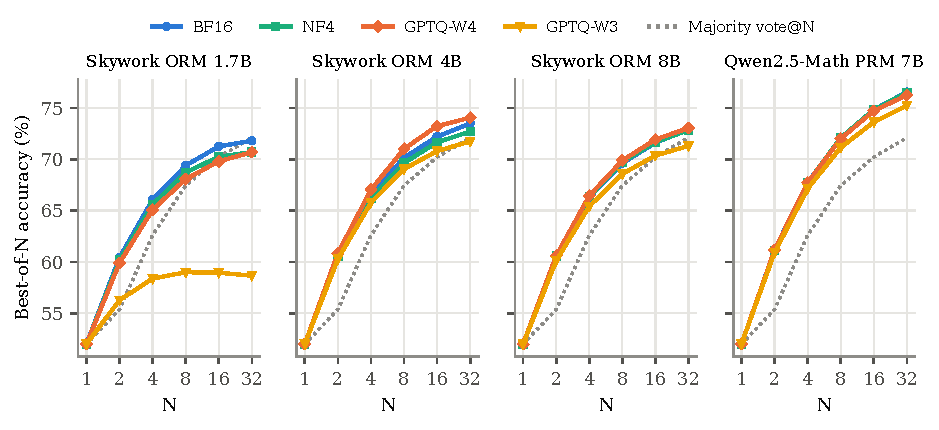
\includegraphics[width=\linewidth]{figures/curves.pdf}
\caption{Best-of-$N$ accuracy as a function of the number of candidates $N$, per
verifier and precision (main study, 2,000 problems; 200 random subsets per problem for
$N<32$). The dotted line is the verifier-free majority vote over the same $N$
candidates.}\label{fig:curves}
\end{figure}

\subsection{Under the 6~GiB verifier budget, the tested 4B 4-bit verifier is best}\label{sec:frontier}

Fig.~\ref{fig:frontier} shows accuracy against measured verifier memory for the tested
deployments. The plan states the ceiling as 6~GB, and we apply it to the GiB
measurements as 6~GiB. The selected configuration needs 4.92~GiB (5.3~GB) and fits under
either reading. The configuration selected on development data is the 4B ORM with packed
GPTQ-W4, and the best BF16 verifier that fits is the 1.7B ORM (4.02~GiB). The
prespecified contrast c2 is $+2.25$\pp\ $[+1.05, +3.45]$ ($p=0.0001$, Holm $p=0.0005$),
so the hypothesis is \textbf{supported}. The 1.7B BF16 verifier is 0.3\pp\ below
majority vote, which needs no verifier, and the 4B GPTQ-W4 verifier is 2.0\pp\ above
it. The comparison applies to the tested checkpoints, the fixed scoring workload and
verifier memory only. In this family accuracy does not grow with size (the 4B BF16
model beats the 8B), so the result describes these deployments and does not imply that
larger verifiers are generally better.

Part of the advantage comes from answer format, and its size depends on the selection
policy. Three secondary analyses, each applied identically to both arms, give a
consistent but smaller effect. With the lenient grader, c2 is $+1.55$\pp\ $[+0.45,
+2.65]$. Restricting Best-of-32 to candidates with an extractable answer gives 75.4\%
versus 74.0\%, a difference of $+1.40$\pp\ $[+0.35, +2.45]$, and a reward-weighted vote
gives 75.5\% versus 74.0\%, $+1.50$\pp\ $[+0.45, +2.55]$. Finally, one of the authors
graded every distinct Best-of-32 winner without an extractable answer in either arm (94
responses), together with 30 random winners with one, without knowing the arm, the
verifier or the grader's verdict (\ref{app:audit}). Replacing the strict grader by these
labels gives $+1.40$\pp\ $[+0.30, +2.50]$ (75.5\% versus 74.1\%, nominal $p=0.011$).
This interval treats the single rater's labels as error-free. None of the three analyses
belongs to the prespecified family. Together they suggest that the deployment advantage
under format-robust grading or selection is about 1.4--1.5\pp, and that the
strict-grader estimate is an upper value. The strict-grader contrast also stays
positive with revised GSM8K labels ($+2.37$\pp) and after excluding truncated
candidates ($+2.20$\pp).

\begin{table}[!htb]
\centering
\small
\caption{Peak verifier memory and scoring throughput on an RTX 4090 (exploratory
re-measurement with a fixed workload of 64 sequences of 900 tokens and no generator
resident). Peak allocated memory is recorded over one pass. Throughput is averaged over
three timed forward passes after one warm-up pass, with GPU synchronisation. The
re-measured peaks match the prespecified measurement used for c2 to within
0.001~GiB. The PRM has no packed GPTQ deployment (Section~\ref{sec:precisions}).}\label{tab:systems}
\begin{tabular}{lrrrrrr}
\toprule
 & \multicolumn{2}{c}{BF16} & \multicolumn{2}{c}{NF4 (\texttt{bitsandbytes})} & \multicolumn{2}{c}{GPTQ-W4 (packed)} \\
verifier & GiB & seq/s & GiB & seq/s & GiB & seq/s \\
\midrule
Skywork-1.7B & 4.02 & 38.0 & 2.13 & 37.6 & 2.07 & 36.7 \\
Skywork-4B & 9.95 & 16.5 & 5.08 & 16.3 & 4.92 & 16.0 \\
Skywork-8B & 16.97 & 9.8 & 7.67 & 9.7 & 7.37 & 9.7 \\
PRM-7B & 16.72 & 11.4 & 7.98 & 11.2 & -- & -- \\
\bottomrule
\end{tabular}
\end{table}

The re-measurement (Table~\ref{tab:systems}) adds the PRM, which needs 16.72~GiB in
BF16 and 7.98~GiB with deployed NF4; the deployed NF4 scores are identical to the
simulated ones. With the PRM included, the best tested deployment under an 8~GiB budget
is the NF4 PRM (76.5\%), ahead of every ORM deployment, while the 6~GiB comparison of c2
is unchanged. Scoring throughput with 4-bit weights was 0.8--3.4\% lower than with BF16.
The workload is a large prefill batch of 57,600 tokens per pass, in which the smaller
weights do not speed up computation and dequantization adds a small cost. We did not
measure small batches, end-to-end latency or a generator resident on the same GPU. For
scale, the generators' BF16 weights alone take about 2.9~GiB (Qwen2.5-1.5B), 6.0~GiB
(Llama-3.2-3B) and 14.2~GiB (Qwen2.5-Math-7B), computed from their parameter counts and
excluding the key--value cache.

\begin{figure}[t]
\centering
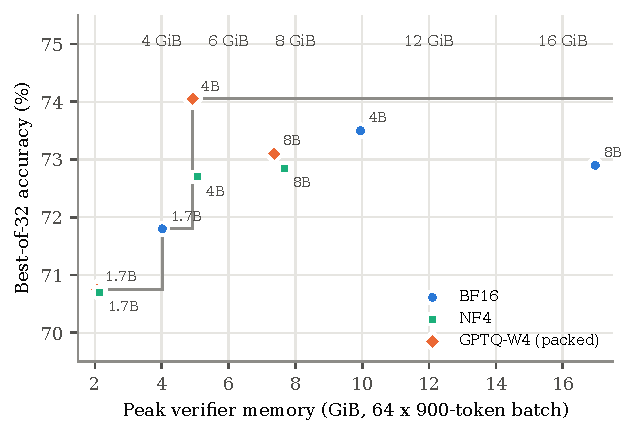
\includegraphics[width=0.75\linewidth]{figures/frontier.pdf}
\caption{Accuracy against measured verifier memory for the tested Skywork ORM and PRM
deployments (Best-of-32, main study, 2,000 problems; PRM memory from the exploratory
re-measurement). Memory is the peak allocation while scoring a fixed workload of 64
sequences of 900 tokens on an RTX 4090 with no generator. GPTQ-W4 uses packed 4-bit
kernels and NF4 uses \texttt{bitsandbytes}. Vertical lines mark the prespecified
ceilings, and the dashed one is the 6~GiB ceiling of c2. The step line is the envelope of
the tested neural-verifier deployments within each budget. Majority vote (dotted) needs
no verifier memory and beats every tested verifier deployment below
4.9~GiB.}\label{fig:frontier}
\end{figure}

\subsection{Selected candidates change often, selected answers much less often}\label{sec:mechanism}

Table~\ref{tab:transitions} breaks the 4-bit and 3-bit changes down into answer
transitions. With GPTQ-W4 or NF4 the selected candidate changes on 21--49\% of
main-study problems, but the selected canonical answer changes on only 4.8--13.2\%, and
72--79\% of the candidate changes keep the same final answer. Harm (a correct BF16
selection becomes wrong) and benefit (the reverse) each affect 0.9--4.1\% of problems
and largely cancel. At 3 bits the answer-change rate (14.2--38.9\%) and harm both grow,
and harm exceeds benefit. H6 and H7 show the same pattern. These measurements are
consistent with answer redundancy in the pools. Candidates that share the selected
answer are interchangeable for accuracy, so most score perturbations move the selection
within the same answer cluster.

\begin{table}[!htb]
\centering
\small
\caption{Answer transitions at $N=32$ relative to BF16 (\% of problems). Cand.: selected
candidate changes; answer: selected canonical answer changes; same: share of candidate
changes that keep the answer; harm: correct $\to$ wrong; benefit: wrong $\to$ correct;
$\Delta_{32}$ = benefit $-$ harm (pp). A switch between two winners without an
extractable answer counts as an answer change. Some such switches are between prose
answers a human would judge equal, so the answer column is an upper value, most of all
for the ORMs that prefer prose answers.}\label{tab:transitions}
\resizebox{\linewidth}{!}{%
\begin{tabular}{lllrrrrrr}
\toprule
study & verifier & condition & cand. & answer & same & harm & benefit & $\Delta_{32}$ \\
\midrule
main & ORM 1.7B & GPTQ-W4 & 48.9 & 13.2 & 73 & 4.1 & 3.0 & $-1.10$ \\
 & & GPTQ-W3 & 87.6 & 38.9 & 56 & 17.7 & 4.5 & $-13.15$ \\
 & ORM 4B & GPTQ-W4 & 29.2 & 8.1 & 72 & 1.7 & 2.3 & $+0.55$ \\
 & & GPTQ-W3 & 59.7 & 17.7 & 70 & 5.2 & 3.5 & $-1.75$ \\
 & ORM 8B & BF16-null & 6.9 & 1.0 & 86 & 0.3 & 0.2 & $-0.10$ \\
 & & NF4 & 21.2 & 4.8 & 78 & 1.3 & 1.2 & $-0.05$ \\
 & & GPTQ-W4 & 25.1 & 6.2 & 76 & 1.5 & 1.7 & $+0.15$ \\
 & & GPTQ-W3 & 50.5 & 14.2 & 72 & 4.3 & 2.7 & $-1.60$ \\
 & PRM & NF4 & 25.2 & 5.7 & 78 & 0.9 & 0.9 & $-0.05$ \\
 & & GPTQ-W4 & 33.0 & 7.1 & 79 & 1.6 & 1.3 & $-0.30$ \\
 & & GPTQ-W3 & 54.0 & 14.3 & 74 & 3.4 & 2.1 & $-1.30$ \\
\midrule
H6 & ORM 8B & GPTQ-W4 & 31.4 & 6.9 & 78 & 1.3 & 1.3 & $0.00$ \\
 & PRM & GPTQ-W4 & 34.4 & 5.8 & 83 & 0.8 & 1.3 & $+0.50$ \\
H7 & ORM 8B & GPTQ-W4 & 26.9 & 8.8 & 67 & 2.1 & 1.8 & $-0.28$ \\
 & PRM & GPTQ-W4 & 30.1 & 8.7 & 71 & 1.0 & 0.5 & $-0.57$ \\
 & ORM 8B & GPTQ-W3 & 51.7 & 20.6 & 60 & 5.8 & 2.3 & $-3.49$ \\
 & PRM & GPTQ-W3 & 55.9 & 20.4 & 64 & 3.8 & 1.2 & $-2.55$ \\
\bottomrule
\end{tabular}}
\end{table}

\begin{figure}[t]
\centering
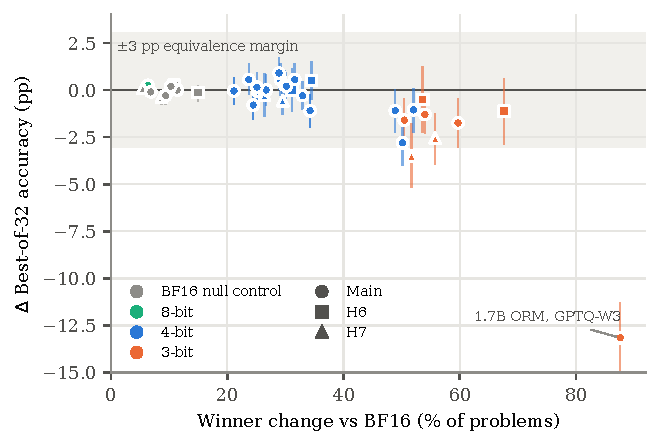
\includegraphics[width=0.75\linewidth]{figures/mechanism.pdf}
\caption{Winner change versus accuracy change at $N=32$ for every quantized condition
and control in the main study (circles) and the two follow-up studies (H6 squares, H7
triangles), with 95\% bootstrap intervals. The exploratory revision experiments
(Llama-based ORMs, in-domain calibration) are not shown. Four-bit conditions change the
selected candidate on 21--52\% of problems, with point estimates inside the $\pm3$\pp\
band. Three-bit conditions change about half or more of the winners and lose
accuracy.}\label{fig:mechanism}
\end{figure}

\subsection{No confirmatory evidence for the MATH-loss and budget-growth contrasts}\label{sec:c4c5}

Development data had suggested that quantization damage concentrates on MATH and grows
with $N$. On the 1,200 evaluation MATH problems, c4 (the MATH $\Delta_{32}$ of the 4B
and 8B ORMs at GPTQ-W4, averaged within problem) is $-0.63$\pp\ $[-1.38, +0.08]$ with
Holm $p=0.40$. c5, the change of that loss from $N=4$ to $N=32$, is $-0.51$\pp\
$[-1.20, +0.16]$ with Holm $p=0.42$. Neither hypothesis is supported. The results are
inconclusive and do not show that the effect is zero, although the intervals rule out
MATH losses larger than about 1.4\pp. c4 measures the loss within MATH and does not test
an interaction with difficulty. The development signal came from 200 problems and did
not replicate.

\subsection{A stronger generator on hard problems (H6)}\label{sec:h6}

H6 tested whether the result holds with a stronger generator on harder, previously
unused problems. Qwen2.5-Math-7B-Instruct \cite{yang2024qwen25math} generated 32
candidates of up to 2,048 tokens for 800 MATH Level-5 test problems, which the 8B ORM and
the PRM scored in BF16 and GPTQ-W4. The family of four tests asked for equivalence at
$\pm3$\pp\ (H6a) and for retention of at least half of the BF16 verifier's advantage
over majority vote (H6b). Let $G = A_{\mathrm{BF16}} - A_{\mathrm{MV}}$ be the BF16
advantage and $\Delta$ the quantization effect. H6b then tests
\[
R \;=\; \tfrac12 G + \Delta \;=\; (A_{\mathrm{Q}} - A_{\mathrm{MV}}) - \tfrac12 G \;>\; 0,
\]
that is, whether the quantized verifier's advantage exceeds half of the BF16 advantage.
$R$ is computed per problem as $R_i = C_{\mathrm{Q},i} - \tfrac12(C_{\mathrm{BF16},i} +
C_{\mathrm{MV},i})$ and bootstrapped as a mean. $R>0$ implies retained value only when
$G>0$, so the plans interpret H6b and H7b only for verifiers with a positive BF16
advantage, which we check descriptively with 97.5\% intervals.

Equivalence is supported for both verifiers, with $\Delta_{32} = 0.00$\pp\ $[-1.13,
+1.13]$ for the ORM and $+0.50$\pp\ $[-0.50, +1.50]$ for the PRM, although the selected
candidate changes on 31\% and 34\% of problems. With this generator, however, neither
verifier showed a clear advantage over majority vote (76.5\%). The PRM tied it ($G =
+0.13$\pp\ $[-1.88, +2.13]$) and the ORM fell below it ($G = -3.75$\pp\ $[-6.25,
-1.25]$). H6 therefore did not establish a positive BF16 advantage to retain, which
limits what its retention tests can show (ORM $R = -1.88$\pp, PRM $+0.56$\pp; neither
supported). These conclusions hold under the lenient grader and without truncated
candidates. Truncation is more common here than in the main study: 19\% of candidates
reached the length limit, all 32 candidates were truncated on 7 of the 800 problems, and
at least three quarters were truncated on 58.

\subsection{Value retention where the verifier adds value (H7)}\label{sec:h7}

H7 is a prospective follow-up targeted at a regime chosen from earlier exploratory
data, namely the main generator on hard problems, where the main-study PRM and 8B ORM had
beaten majority vote. It uses all 1,060 MATH Level-4 and Level-5 test problems not used
anywhere else in this work, the prespecified generation settings, and the same
verifiers, conditions, tests and analysis code as H6. Because the regime was chosen with
knowledge of earlier results, H7 estimates the effect of quantization in that regime. It
does not estimate the typical value of a verifier across deployments.

On the new problems both verifiers beat majority vote in BF16, the PRM by $+8.2$\pp\
(97.5\% interval $[+5.9, +10.7]$) and the 8B ORM by $+3.0$\pp\ $[+0.4, +5.8]$. All four
prespecified hypotheses are supported (Holm over four). Accuracy is equivalent at
$\pm3$\pp, with $\Delta_{32} = -0.28$\pp\ $[-1.42, +0.85]$ for the ORM and $-0.57$\pp\
$[-1.32, +0.19]$ for the PRM. Both quantized verifiers keep more than half of their BF16
advantage. The evidence is strong for the PRM ($R = +3.54$\pp\ $[+2.45, +4.72]$, Holm
$p \le 0.0003$) and narrow for the ORM ($R = +1.23$\pp\ $[-0.14, +2.59]$, one-sided Holm
$p = 0.041$), in line with the ORM's lower planned power. Descriptively, the PRM retains
93\% of its advantage (95\% interval 84--102\%) and the ORM 91\% (44--149\%). The ORM's
interval is wide because its BF16 advantage, the denominator of the ratio, is small. The
retention conclusions keep their sign under the lenient grader and without truncated
candidates, which the plan required before describing value as preserved. In an
exploratory comparison, three bits is not safe in this regime: GPTQ-W3 costs $3.5$\pp\
for the ORM and $2.6$\pp\ for the PRM and removes the ORM's advantage. Level-wise
estimates and all sensitivity analyses are in the repository, and
Fig.~\ref{fig:retention} summarises the advantage over majority vote before and after
quantization across regimes.

\begin{figure}[t]
\centering
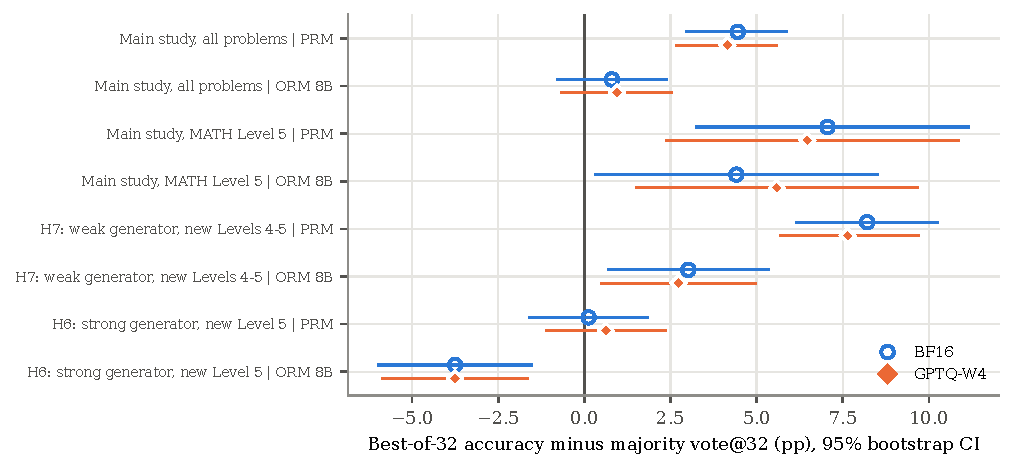
\includegraphics[width=\linewidth]{figures/retention.pdf}
\caption{Verifier advantage over majority vote (Best-of-32 accuracy minus majority
vote@32, pp, with 95\% bootstrap intervals) in BF16 (open circles) and with GPTQ-W4
(diamonds), for the 8B ORM and the PRM. Main-study rows are exploratory subsets; H6 and
H7 are separately planned studies on new problems.}\label{fig:retention}
\end{figure}

\subsection{Robustness and controls}\label{sec:robustness}

\paragraph{Other reward-model families} As an exploratory extension, we scored the
previously analysed main and H7 pools with two further ORMs on a Llama~3.1 backbone
(Table~\ref{tab:otherrm}). The 4-bit result holds within the $\pm3$\pp\ margin, with
somewhat larger losses than for the Skywork-Qwen models. GPTQ-W4 changes the accuracy of
Llama-3.1-Tulu-3-8B-RM by $-0.60$\pp\ on the main problems and $-0.75$\pp\ on H7, and
that of Skywork-Reward-V2-Llama-3.1-8B by $-1.45$\pp\ and $-1.23$\pp. All four 90\%
intervals lie inside $\pm3$\pp, but the Skywork-Llama loss on the main problems is
distinguishable from zero. Both models changed the selected candidate (44--53\%) and the
selected answer (11--25\%) more often than the Skywork-Qwen ORMs. Neither showed a clear
advantage $G$ over majority vote in BF16, so value retention cannot be interpreted for
them. With generic calibration at 3 bits, both Llama-based models break down. GPTQ-W3
costs Tulu-3 $12.6$\pp\ and Skywork-Llama $26.4$\pp, which puts the latter below the
random-candidate rate, against $1.6$\pp\ for the Qwen-based 8B ORM. With generic
calibration the 3-bit behaviour is therefore strongly model-dependent; for Tulu-3,
in-domain calibration recovers most of the loss (next paragraph).

\begin{table}[!htb]
\centering
\small
\caption{Exploratory results for the two Llama-3.1-based ORMs (Best-of-32). $A$: BF16
accuracy (\%); $\Delta$: change with GPTQ-W4 (pp) with 95\% and 90\% intervals; $G$:
BF16 advantage over majority vote (pp, 95\% interval; majority vote 72.1\% on the main
problems and 55.9\% on H7); cand./answer: share of problems whose selected candidate or
answer changes (\%). GPTQ-W3 with generic calibration on the main problems: Tulu-3
$-12.60$ $[-14.40, -10.75]$, answer change 35\%; Skywork-Llama $-26.35$ $[-28.70,
-24.05]$, answer change 59\%.}\label{tab:otherrm}
\resizebox{\linewidth}{!}{%
\begin{tabular}{llrrrrrr}
\toprule
ORM & population & $A$ & $\Delta$ [95\% CI] & 90\% CI & $G$ [95\% CI] & cand. & answer \\
\midrule
Tulu-3-8B-RM & main (2,000) & 72.5 & $-0.60$ [$-1.65$, $+0.45$] & [$-1.45$, $+0.30$] & $+0.35$ [$-1.20$, $+1.85$] & 44.6 & 11.5 \\
 & H7 (1,060) & 55.0 & $-0.75$ [$-2.45$, $+0.85$] & [$-2.17$, $+0.57$] & $-0.94$ [$-3.11$, $+1.23$] & 43.6 & 18.3 \\
Skywork-Llama-8B & main (2,000) & 68.8 & $-1.45$ [$-2.75$, $-0.15$] & [$-2.55$, $-0.35$] & $-3.35$ [$-5.05$, $-1.65$] & 51.7 & 18.3 \\
 & H7 (1,060) & 53.8 & $-1.23$ [$-3.11$, $+0.66$] & [$-2.74$, $+0.38$] & $-2.17$ [$-4.62$, $+0.28$] & 53.2 & 24.7 \\
\bottomrule
\end{tabular}}
\end{table}

\paragraph{Task-matched calibration at 3 bits} Much of the 3-bit loss depends on the
calibration data (exploratory; Table~\ref{tab:calib}). The prespecified recipe uses 128
WikiText chunks of exactly 512 tokens. The in-domain alternative uses 128 complete
candidate responses sampled from the generator's development pools, in the verifier's
input format and of variable length (about 490--540 tokens on average, depending on the
tokenizer). The calibration problems are development problems, disjoint from the
evaluation set. With the in-domain recipe, the loss of the 1.7B ORM falls from
$13.15$ to $3.75$\pp, and that of Tulu-3, a Llama-based ORM, from $12.60$ to $2.80$\pp.
The recoveries are $+9.40$\pp\ and $+9.80$\pp. For the verifiers that lost little with
generic calibration the change is smaller: $+1.55$\pp\ for the 8B ORM and $+0.70$\pp\
$[-0.35, +1.75]$ for the PRM, whose interval includes zero. A length control rules out
sequence length as the explanation. Calibrating the 1.7B ORM on WikiText cut to exactly
the token lengths of its in-domain set gives $\Delta_{32} = -16.75$\pp, no better than
the generic recipe and $13.00$\pp\ $[11.00, 14.95]$ worse than in-domain calibration.
The recovery therefore comes from the content of the calibration text, its domain or
its format, which this design does not separate. For the tested verifiers, the 3-bit
boundary we observe depends on the calibration recipe as well as on the bit width.
Skywork-Llama was not re-quantized with the in-domain recipe.

\begin{table}[!htb]
\centering
\small
\caption{GPTQ-W3 with generic and in-domain calibration (exploratory, main study, 2,000
problems, Best-of-32). $\Delta_{32}$ versus BF16 and the paired difference, in pp with
95\% intervals. Length control for the 1.7B ORM: WikiText cut to the token lengths of
its in-domain set, $\Delta_{32} = -16.75$ $[-18.75, -14.80]$.}\label{tab:calib}
\resizebox{\linewidth}{!}{%
\begin{tabular}{lrrrr}
\toprule
verifier & BF16 $A_{32}$ (\%) & generic $\Delta_{32}$ & in-domain $\Delta_{32}$ & in-domain $-$ generic \\
\midrule
Skywork-1.7B & 71.8 & $-13.15$ [$-15.05$, $-11.25$] & $-3.75$ [$-5.25$, $-2.30$] & $+9.40$ [$+7.55$, $+11.30$] \\
Skywork-8B & 72.9 & $-1.60$ [$-2.75$, $-0.45$] & $-0.05$ [$-1.00$, $+0.90$] & $+1.55$ [$+0.40$, $+2.75$] \\
PRM-7B & 76.6 & $-1.30$ [$-2.30$, $-0.25$] & $-0.60$ [$-1.45$, $+0.25$] & $+0.70$ [$-0.35$, $+1.75$] \\
Tulu-3-8B-RM & 72.5 & $-12.60$ [$-14.40$, $-10.75$] & $-2.80$ [$-4.00$, $-1.65$] & $+9.80$ [$+7.95$, $+11.60$] \\
\bottomrule
\end{tabular}}
\end{table}

\paragraph{Selection rules} The 4-bit result does not depend on the selection rule
(exploratory, main study, $N=32$). In the reward-weighted answer vote each candidate
with an extractable answer adds $\mathrm{softmax}(s/T)$ to its answer cluster, where $s$
is the verifier score and $T$ is fitted on development data in BF16 and kept fixed
across precisions ($T=0.3$ for the 8B ORM and $0.1$ for the other verifiers). Under
reward-weighted voting, BF16 accuracy and its change with GPTQ-W4 are 73.95\%
($-1.00$\pp) for the 1.7B ORM, 76.00\% ($-0.60$\pp) for the 4B ORM, 76.20\%
($+0.30$\pp) for the 8B ORM and 79.50\% ($+0.25$\pp) for the PRM. Restricting
Best-of-32 to candidates with an extractable answer gives 73.95\% ($-1.10$\pp), 75.95\%
($-0.55$\pp), 76.10\% ($0.00$\pp) and 79.75\% ($-0.45$\pp) for the same four verifiers,
and last-step aggregation for the PRM gives 79.35\% ($-0.25$\pp). GPTQ-W3 loses
0.7--11\pp\ under every rule. Restricting selection to extractable answers raises the
BF16 ORMs' accuracy by 2.2--3.2\pp\ (for the 8B ORM, from 72.9\% to 76.1\%), which shows
how much the strict grader penalises their preference for prose answers. Under both
rules the c2 contrast stays positive ($+1.40$ and $+1.50$\pp;
Section~\ref{sec:frontier}).

\paragraph{Answer format} Under the strict grader several quantized conditions appeared
to \emph{improve} GSM8K accuracy, for example by $+3.0$\pp\ for the 4B ORM at GPTQ-W4
and by $+8.0$\pp\ on the Llama pools. The format/content decomposition
(Section~\ref{sec:grading}) shows that these gains come from answer format. Quantization
weakens the Skywork ORMs' preference for prose answers without a boxed final answer. For
the 4B ORM at GPTQ-W4 the format term is $+3.0$\pp\ and the content term $0.0$\pp, and
the difference under the lenient grader is $+0.4$\pp. On MATH the changes come from
answer content under both graders. We therefore claim no accuracy gain from
quantization.

\paragraph{Packed versus simulated quantization} Packed GPTQ-W4, which runs FP16 Marlin
kernels, and simulated GPTQ-W4, which runs in BF16, select the same final answer on
98.8--99.2\% of problems and the same candidate on 84.7--88.8\%. Their candidate-level
disagreement (11.3--15.4\%) is somewhat larger than the bf16-null floor (6.9--11\%), and
their answer-level disagreement (0.8--1.2\%) is of the same size as the null control's
(1.0\% for the 8B ORM). Correctness flips are rare and symmetric (0.35--0.55\% of
problems). Packed GPTQ-W4 changes accuracy versus BF16 by $-1.05$, $+0.55$ and
$+0.20$\pp\ for the 1.7B, 4B and 8B ORMs, against $-1.10$, $+0.55$ and $+0.15$\pp\ for
simulated quantization. c2 uses the packed scores.

\paragraph{Second generator} On 300 problems with Llama-3.2-3B-Instruct candidates
(exploratory), GPTQ-W4 changes the PRM's Best-of-32 accuracy by $+0.33$\pp\ $[-3.00,
+4.00]$ and NF4 by $-0.67$\pp. For the 4B ORM the strict grader shows $+8.0$\pp, which
shrinks to $+2.0$\pp\ $[0.0, +4.3]$ under the lenient grader, again a format effect.
With this generator, majority vote (76.3\%) beats both verifiers in BF16 (ORM 63.7\%,
PRM 70.7\%).

\paragraph{Labels and truncation} With GSM8K-Platinum labels the c1 estimate is
$+0.44$\pp. c4 and c5 involve MATH only and do not change. With truncated candidates
removed before selection, the estimates are $+0.33$\pp\ for c1, $-0.67$\pp\ for c4 and
$-0.52$\pp\ for c5. None of these sensitivity estimates reverses the direction of a
prespecified conclusion. Both GSM8K problems whose labels the human audit had flagged as
questionable are among those that GSM8K-Platinum removes.

\section{Discussion}\label{sec:discussion}

\paragraph{Deployment guidance.} For reward-model verifiers of 4B parameters and above,
4-bit weight quantization (GPTQ, AWQ or NF4) is a safe default for Best-of-$N$
selection on mathematical problems: across three preregistered settings, two
generators, an ORM family and a PRM, the accuracy change stayed within about 1.5\pp\
and the verifier's advantage over majority vote was largely preserved. Under a fixed
memory budget, the freed memory is better spent on a larger quantized verifier than on
a smaller full-precision one (c2). Three bits is not a safe default: it is harmless in
some regimes (H6) but costs 2--4\pp\ in others (H7, main study) and is catastrophic for
the 1.7B ORM, and the smallest verifier is also sensitive to the quantization method
(RTN versus GPTQ).

\paragraph{Why quantization rarely matters, and when it could.} Best-of-$N$ only needs
the top of the ranking to keep a correct answer, and candidate pools are redundant:
many candidates share the same final answer. Quantization perturbs scores enough to
change the selected candidate on a quarter to a third of problems, yet the new winner
usually carries the same answer. The risk is concentrated on contested problems, where
competing answers have similar support and the verifier's preference is what decides;
there, coarse quantization does tip choices (3 bits), and in our H6 and H7 data the
perturbation tends to move the selection towards the consensus answer. This suggests
that quantization damage should grow with the share of contested problems and with how
much a verifier's decisions depart from the consensus, rather than with nominal
difficulty or with $N$, which is consistent with our unsupported difficulty and budget
hypotheses (c4, c5).

\paragraph{How much a verifier is worth.} The question ``does quantization destroy the
value a verifier adds?'' presupposes that the verifier adds value. With the weak
generator the Skywork ORMs were within about one point of majority vote overall, and
with a strong math generator on hard problems majority vote matched the PRM and beat the
ORM by 3.8\pp. Only in a regime selected for verifier advantage (H7) did both verifiers
clearly beat majority vote. Practitioners should measure a verifier against
self-consistency on their own generator before paying its memory and latency cost.

\paragraph{Evaluating selection.} Three practices changed our conclusions or their
size. (i) A strict answer grader turned a reward-model preference for prose answers into
apparent quantization ``gains'' of up to 8\pp; a format/content decomposition and a
lenient grader removed them, and exhaustive blinded human grading reduced the registered
memory-frontier effect from 2.25 to 1.4\pp. (ii) A fixed-precision null control (same
weights, different batch layout) changes 5--15\% of winners across our studies; winner-change rates without
such a floor overstate instability. (iii) Development-set signals that motivated two
registered hypotheses did not replicate on 1,200 evaluation problems; preregistering
them made the non-replication visible rather than leaving it in a file drawer.

\paragraph{Limitations.} The ORMs come from a single family (Skywork-Reward-V2, built on
Qwen3), the PRM is a Qwen model and the generators are Qwen and Llama models, so
family-specific robustness cannot be excluded. Accuracy experiments use simulated
quantization; packed 4-bit kernels agreed with it on 98.8--99.2\% of selected answers,
but we measured memory, not latency or throughput. The tasks are GSM8K and MATH, whose
test problems may have been seen during pre-training of the generators and verifiers;
contamination affects BF16 and quantized verifiers equally because both score the same
frozen pools, but it can change pool redundancy and verifier advantage. Candidates were
capped at 1,024 or 2,048 tokens, and 6.5--19\% reached the cap, although excluding them
does not change any conclusion. The value-retention result is confirmatory for the PRM
and only narrowly so for the ORM, and we did not find a strong-generator regime in which
the verifiers clearly beat majority vote, so retention of a large advantage under a
strong generator remains untested. The analysis plans were fixed in version control
before the corresponding data were generated or scored; we did not use an external
registry.

\section{Conclusion}\label{sec:conclusion}

We asked whether the reward-model verifier in Best-of-$N$ mathematical answer selection
can be quantized without losing what it is for. On frozen candidate pools, with analysis
plans fixed before the data, the answer is yes at 4 bits for verifiers of 4B parameters
and above: GPTQ-W4 keeps Best-of-32 accuracy within a $\pm3$\pp\ equivalence margin in
the main study and in two follow-up studies with a stronger generator and with new hard
problems, and where the verifier beats majority vote it keeps most of that advantage
(93\% for the PRM). Under a fixed memory budget a larger quantized verifier is the better
choice. Robustness comes from the selection task rather than from score fidelity:
quantization changes the selected candidate often, but pools are redundant, so the
selected answer rarely changes; 3-bit weights and the smallest verifier are where this
breaks down. Two practical caveats travel with these results. Measure a verifier against
majority vote on one's own generator, because with a strong generator it may add
nothing; and evaluate selection with a grader that is robust to answer format, because a
strict grader can turn format preferences into spurious effects of quantization.

\section*{CRediT authorship contribution statement}

\textbf{Hector Borobia:} Writing -- review \& editing, Writing -- original draft,
Visualization, Validation, Software, Project administration, Methodology,
Investigation, Formal analysis, Data curation, Conceptualization. \textbf{Elies
Segu\'{i}-Mas:} Writing -- review \& editing, Supervision. \textbf{Guillermina
Tormo-Carb\'{o}:} Writing -- review \& editing, Supervision.

\section*{Declaration of Generative AI and AI-assisted technologies in the writing
process}

During the preparation of this work, the authors used Claude Code (Anthropic) to support
code development, language editing, and consistency checking. After using this tool, the
authors reviewed and edited the content as needed and take full responsibility for the
content of the published article.

\section*{Funding}

This research did not receive any specific grant from funding agencies in the public,
commercial, or not-for-profit sectors.

\section*{Declaration of competing interest}

The authors declare that they have no known competing financial interests or personal
relationships that could have appeared to influence the work reported in this paper.

\section*{Data availability}

Code, configuration, frozen problem manifests, analysis plans with their amendments,
analysis scripts and figure-generation scripts are available at the project repository:
\todo{https://github.com/hecboar/quantized-verifiers-bon (tag v1.0-submission)}. The
candidate pools and all verifier scores are available at
\todo{Hugging Face dataset URL}.


\bibliographystyle{elsarticle-num}
\bibliography{references}

\appendix
\section{Implementation details}\label{app:impl}

\paragraph{Prompt} Every generator receives the system prompt ``Please reason step by
step, and put your final answer within \texttt{\textbackslash boxed\{\}}.'' and the
problem as the user turn, through its chat template. For Llama-3.2-3B the instruction is
repeated at the end of the user turn. This is a recorded deviation: without the
repetition, 34\% of its candidates had no extractable answer.

\paragraph{Verifier inputs} The ORMs (Skywork-Reward-V2-Qwen3 1.7B/4B/8B,
Skywork-Reward-V2-Llama-3.1-8B, Llama-3.1-Tulu-3-8B-RM) receive the (problem, response)
pair as a user/assistant conversation formatted by their chat template, without a system
prompt and with a single beginning-of-sequence token. They output a scalar from their
reward head, and we verified that the padding token never appears inside a sequence.
Tulu-3-8B-RM does not define a padding token ID in its model configuration, so we assign
the tokenizer's padding token ID. The PRM receives its documented system prompt, the
problem, and the response split into steps at blank lines and separated by its step
token. Its score is the minimum step reward, and the last-step reward is stored for the
sensitivity analysis.

\paragraph{Quantization} All linear layers inside the transformer blocks are quantized
(weight-only), while embeddings, norms, the reward head and activations stay in BF16.
GPTQ uses group size 128, symmetric quantization and 1\% diagonal damping, and it is
calibrated on 128 WikiText-2 sequences of 512 tokens drawn with a fixed seed. AWQ uses
the same calibration and group size, NF4 uses \texttt{bitsandbytes} without double
quantization, and RTN uses group size 128 at 4 bits and per-channel scales at 8 bits. We
audit every quantized model by fingerprinting all parameters before and after
quantization. Every target layer must change (for example 252 of 252 for the 8B ORM and
196 of 196 for the PRM), and no other parameter may change.

\paragraph{PRM rotary buffers}\label{app:prm} With \texttt{transformers} 5.x, the remote
modelling code of Qwen2.5-Math-PRM-7B is instantiated on the meta device, and its
non-persistent rotary-embedding buffers come back uninitialised after loading. Scores
computed this way were below the random-candidate rate. We recompute the buffers exactly
as the model's own initialisation does and check them at every load. All PRM results in
this paper use repaired buffers, and the affected scores were discarded (a recorded
deviation).

\paragraph{Software and compute} Generation used vLLM 0.30.0. Scoring used PyTorch
2.13.0 (CUDA 13.0) with \texttt{transformers} 5.17 in the main study and 5.19 in the
follow-up studies, and the packed kernels used \texttt{gptqmodel}. Model identifiers and
all settings are recorded in the repository and in the metadata of every score file.
All experiments ran on single cloud GPUs, mostly RTX 4090, with some follow-up runs on
L40S and other GPUs with at least 24~GB. The BF16 and quantized runs of a verifier
always used the same GPU. The total was roughly 90 GPU-hours, including setup.

\section{Blinded audit of the outcome measure}\label{app:audit}

A human rater (one of the authors) inspected all 94 distinct Best-of-32 winners without
an extractable final answer in either arm of the memory-budget contrast c2 (48 from the
4B GPTQ-W4 arm and 68 from the 1.7B BF16 arm, with 22 shared), together with 30 randomly
sampled winners that had an extractable answer. Each item showed only the problem, the
reference answer and the full response, typeset as mathematics. The endpoint was
final-answer correctness. Responses that reached the length limit were marked as such
and checked individually, and by a rule fixed beforehand they counted as incorrect when
they stopped before stating a final answer. Of the 24 truncated responses audited, 23
were judged incorrect. The remaining one (R079) had stated its final answer before the
cut and was judged correct.

The rater judged 83 responses correct, 29 incorrect and 12 unsure. In a blinded second
pass, with the same view and before opening the key, the rater re-examined every unsure
and incorrect verdict. The pass confirmed all 29 incorrect verdicts and resolved all 12
unsure ones as incorrect: 11 had been cut by the length limit before giving a final
answer, 3 of them on a correct track, and one had a wrong final answer. It also flagged
two GSM8K problems with questionable reference labels, both of which GSM8K-Platinum
removes. If the first-pass verdicts are used and the unsure items dropped, the corrected
c2 is $+1.41$\pp\ $[+0.35, +2.46]$ instead of $+1.40$. On the 30 controls the strict
grader and the human agree on 29. On the 94 winners without an extractable answer the
strict grader scores all as wrong, while the human judges 60 correct (27 of 48 in the 4B
arm, 45 of 68 in the 1.7B arm and 12 of the 22 shared), and the lenient grader agrees
with the human on 85. The audit covers all such winners plus 30 controls and was done by
a single rater, so grading error among winners with an extractable answer is measured
only on the 30 controls.

\section{Analysis plans and deviations}\label{app:deviations}

Table~\ref{tab:chronology} lists the chronology recorded in the repository. All
deviations are documented with dates. In the main study, the formatting instruction was
repeated in the Llama prompt, and the PRM rotary buffers were repaired before rescoring.
The prespecified decision rule permitted running c3, whose calibration hyper-parameter
had been frozen on development data. At the prespecified 4 bits, however, the 8B ORM
showed no MATH damage to repair, so c3 was not run and stays in the family with $p=1$.
After the main results we added the exploratory bit-width dose-response runs and
included the packed 1.7B model in the memory frontier. In H6 the first candidate pool
was lost before inspection and regenerated, and scoring was split across four GPUs. In
H7, GPUs other than the RTX 4090 had to be used because of limited availability, and the
lenient-grader verdicts were computed with time limits equivalent to those on Linux. The
corrections to the follow-up analysis script were made before H7 data existed and
reproduce all H6 results exactly. The exploratory revision experiments (additional
reward models, task-matched 3-bit calibration, and the memory and throughput
re-measurement), and the second set (in-domain 3-bit calibration for the PRM and Tulu-3,
and the length control), were specified before their launch.

One analysis correction was made after the main results. The exploratory majority-vote
baseline of the main study had broken ties between answer clusters by verifier score,
and it fell back to the Best-of-$N$ winner when no candidate had an extractable answer.
On 14 October (commit \texttt{8a69567}) it was replaced by the verifier-independent rule
of Section~\ref{sec:selection}. The change affects the majority outcome on 12--14 of the
2,000 main-study problems (72.4--72.7\% becomes 72.1\%) and only exploratory main-study
tables and figures. The H6 and H7 analyses always used the verifier-independent rule, so
no confirmatory test, gain $G$ or retention statistic $R$ changes.

\begin{table}[!htb]
\centering
\scriptsize
\caption{Chronology of plans and data (commit timestamps, 2026).}\label{tab:chronology}
\resizebox{\linewidth}{!}{%
\begin{tabular}{lll}
\toprule
date & event & data existing at that point \\
\midrule
27 Sep & plan (c1--c3); manifests frozen & none \\
27--28 Sep & go/no-go gate on development problems & dev.\ scores \\
28 Sep 11:20 & amendment 1: c4, c5, MATH extension & dev.\ scores \\
28 Sep 11:43--14:00 & main-study pools generated & candidates$^{a}$ \\
28 Sep 14:17 & amendment 2: populations, tests, c3 rule, hashes & candidates$^{a}$ \\
from 28 Sep 14:17 & main-study scoring and analysis & -- \\
12 Oct 19:00 & H6 plan, manifests, analysis code & none \\
13 Oct 02:10 & H6 pool hashes; then scoring & candidates \\
13 Oct 13:17 & H7 plan (same analysis code) & none \\
13 Oct 14:27 & H7 pool hashes; then scoring & candidates \\
14 Oct 00:08 & majority-vote tie rule corrected (exploratory tables) & all main scores \\
14 Oct 00:14 & revision experiments fixed (exploratory) & none of the new runs \\
\bottomrule
\end{tabular}}

\smallskip
\raggedright\scriptsize $^{a}$Generator statistics only (accuracy, extractable answers, truncation); no verifier score.
\end{table}


\end{document}
